\subsection{Representaci\'on por medio de un circuito l\'ogico}

\noindent
A partir de las expresiones \ref{ecy0},  \ref{ecy1}, \ref{ecy2}, y \ref{ecy3}, se pudo plantear el comportamiento a trav\'es de un circuito l\'ogico. Para ello, se tomaron compuertas del tipo AND, OR y NOT. A continuaci\'on se expone dicho esquema.

\begin{figure}[h!]
    \centering
    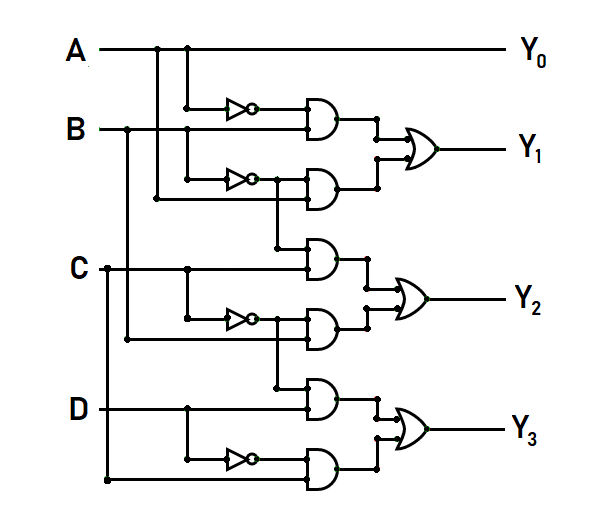
\includegraphics[scale=0.6]{images/ej4/logiccircuitej4.png}
    \caption{Representaci\'on de las expresiones mediante un circuito l\'ogico}
    \label{fig:circuito4fig}
\end{figure}

\noindent
El circuito esquematizado en la figura \ref{fig:circuito4fig} es el resultado de expresiones del tipo de suma de productos. Este factor se puede observar en el diagrama debido a que, excepto en $Y_0$ su valor es directamente equivalente al de A, las salidas parten inmediatamente despu\'es de una compuerta OR cuyas entradas siempre son las salidas de dos compuertas AND. 